%!TEX root = practicum1.tex

\begin{figure}
	\centering
	\begin{subfigure}{0.9\columnwidth}
		\centering
		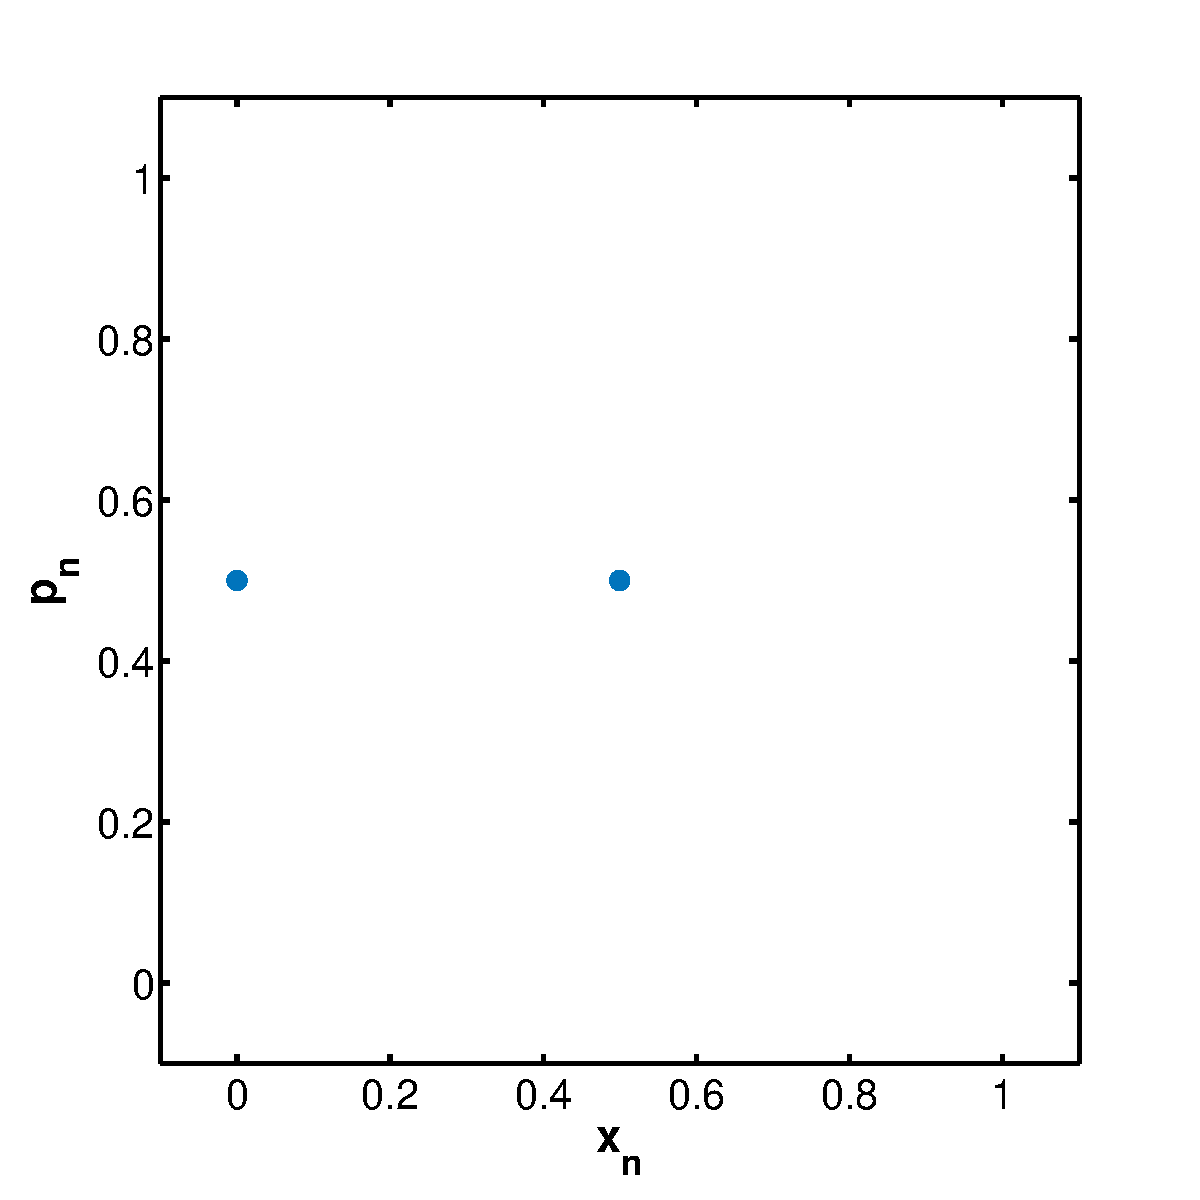
\includegraphics[width=\textwidth]{./img/assignment_a_0_dim}
		\caption{$x_n = 0.5, p_n = 0.5$}
		\label{fig:experiment:dimension:zero}
	\end{subfigure}

	\begin{subfigure}{0.9\columnwidth}
		\centering
		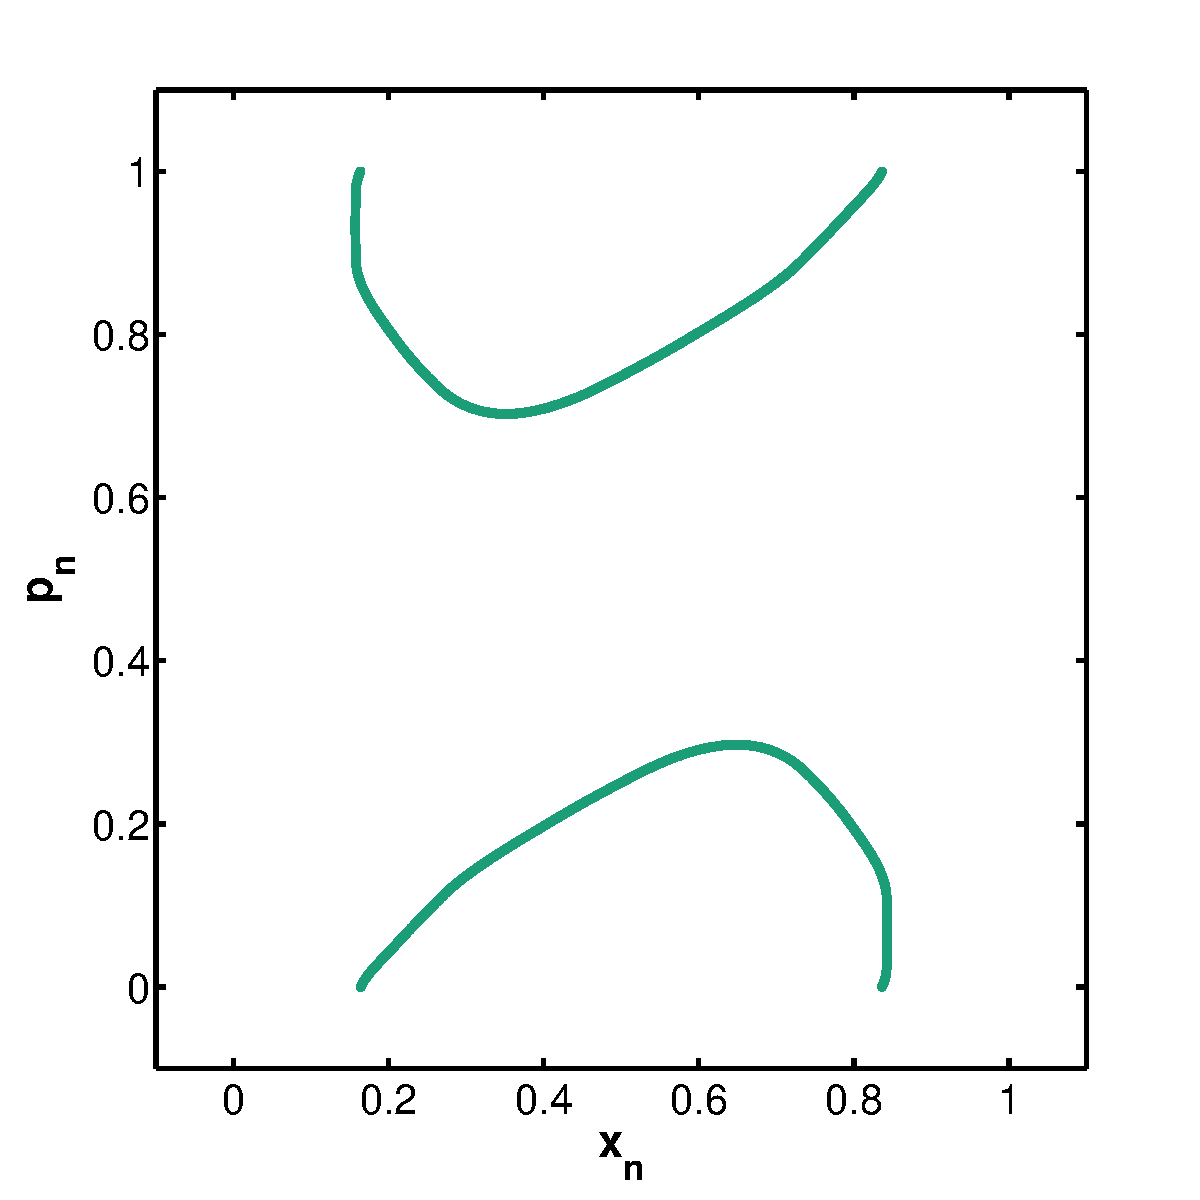
\includegraphics[width=\textwidth]{./img/assignment_a_1_dim}
		\caption{$x_n = \num{0.1576131}, p_n = \num{0.9705928}$}
		\label{fig:experiment:dimension:one}
	\end{subfigure}

	\begin{subfigure}{0.9\columnwidth}
		\centering
		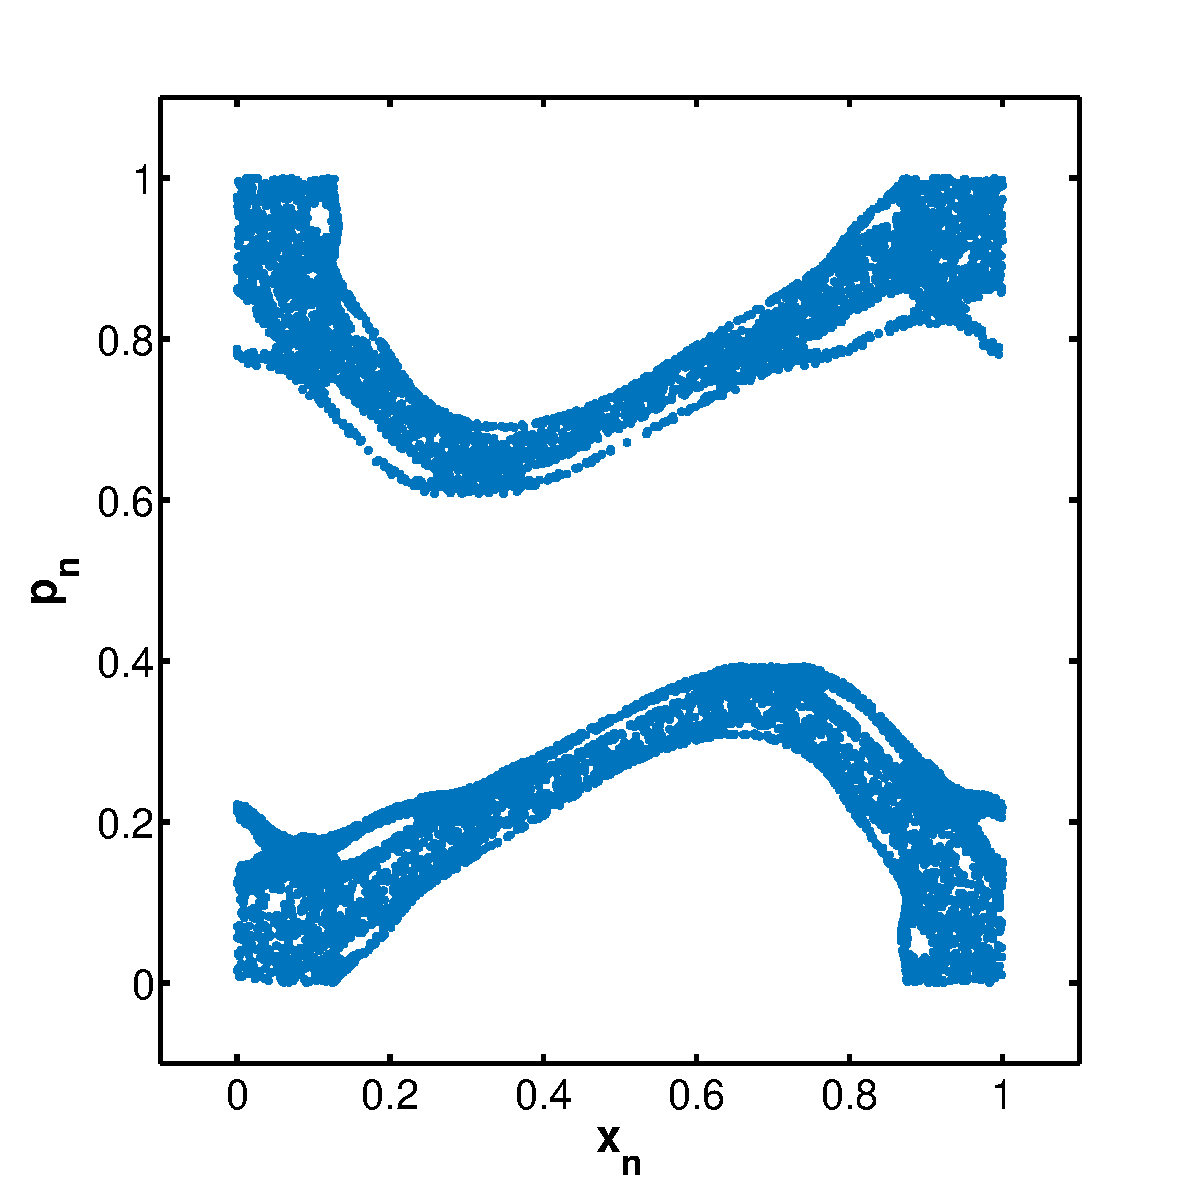
\includegraphics[width=\textwidth]{./img/assignment_a_2_dim}
		\caption{$x_n = \num{0.1269868}, p_n = \num{0.9133759}$}
		\label{fig:experiment:dimension:two}
	\end{subfigure}
	\caption{}
	\label{fig:experiment:dimension}
\end{figure}
